\documentclass[a0,portrait]{a0poster}
\usepackage{graphicx}
\usepackage{multicol}
\usepackage{charter}
\usepackage{color}
\usepackage[utf8]{inputenc}
\usepackage{amsmath}
\usepackage{caption}
\usepackage{enumitem}
\usepackage{booktabs}
\usepackage{xcolor}
\usepackage{array}
\usepackage{parskip}          % Activa el paquete para controlar el espacio entre párrafos
\usepackage{comment} %sirve para agregar comentarios en mas de una línea del código
\usepackage{tcolorbox}


\renewcommand{\figurename}{Gráfico}
\renewcommand{\tablename}{Tabla}
\definecolor{miRojo}{rgb}{0.82, 0.32, 0.31}  % Definir el color usando valores rgb
\definecolor{lightgray}{gray}{0.9}  % Color gris claro para subrayado
\definecolor{miGray}{gray}{.6}  % Color gris claro para subrayado
\definecolor{miVerde}{rgb}{0.0, 0.6, 0.0}  % Definir un color verde personalizado
\setlength{\parindent}{2em}   % Ajusta la sangría global
\setlength{\parskip}{2em}     % Ajusta el espacio entre párrafos
\captionsetup{font=footnotesize}  % Cambia el tamaño del nombre del gráfico y la leyenda

\setlength{\columnsep}{2cm}
\setlength{\columnseprule}{2.5pt}
\def\columnseprulecolor{\color{miRojo}}


% Crear comando para secciones subrayadas y centradas con cuadro rojo
\newcommand{\customsection}[1]{
    \begin{center}
        \begin{tcolorbox}[colframe=miRojo!50, colback=miRojo, width=\linewidth, boxrule=1mm, arc=3mm, auto outer arc]
            \centering
            \vspace{.5cm} % Espacio entre el parrafo anterior y el subtitulo
            \color{white}
            \section*{ \textbf{\Huge #1}}  % El título se sigue mostrando con el diseño original
            \vspace{.2cm} % Espacio después del título
        \end{tcolorbox}
    \end{center}
}

\begin{document}
% Recuadro inicial en todo el ancho de la hoja sin márgenes
\begin{tcolorbox}[colframe=miGray, colback=miGray!40, width=\linewidth, boxrule=1mm, arc=3mm, left=0pt, right=0pt, top=0pt, 
    bottom=0pt, boxsep=0pt]
    \centering
        
\includegraphics[width=.3\linewidth]{logo_fae_web.png}\\
        \vspace{-2.5cm} % Ajusta este valor si es necesario para el espaciado
        \VeryHuge \textbf{\emph{Evaluación del poder predictivo de estrategias técnicas de tendencia y momentum sobre acciones 
        americanas}}\par
        \vspace{1cm}
        \Huge Mateo Canales Briceño, Cristóbal González Araya, Tomás Leyton Muñoz \par
        \LARGE Escuela de Ingeniería Comercial, Universidad Diego Portales, 2024 \par
        \vspace{1cm}

\end{tcolorbox}

\vspace{2cm}


\begin{multicols}{2}
    % Sección 1: 
    \customsection{Highligths}
    \begin{multicols}{2}
            \begin{itemize}
                \item Los puntos más importantes de esta investigación son:
                \begin{itemize}
                    \item Los indicadores técnicos por si solos no tienen mejores resultados que las acciones y son poco significativos.
                    \item Los indicadores técnicos tienen porcentaje de éxito mayor en aquellas empresas que han sostenido un crecimiento constante en sus retornos durante los últimos 5 años.
                    \item La aplicación de varios indicadores mejora la significancia al momento de ser aplicar la estrategia.
                    
                \end{itemize}
            \end{itemize}
            \columnbreak
             % Gráfico con minipage  
    \begin{minipage}{\linewidth}
        \centering
        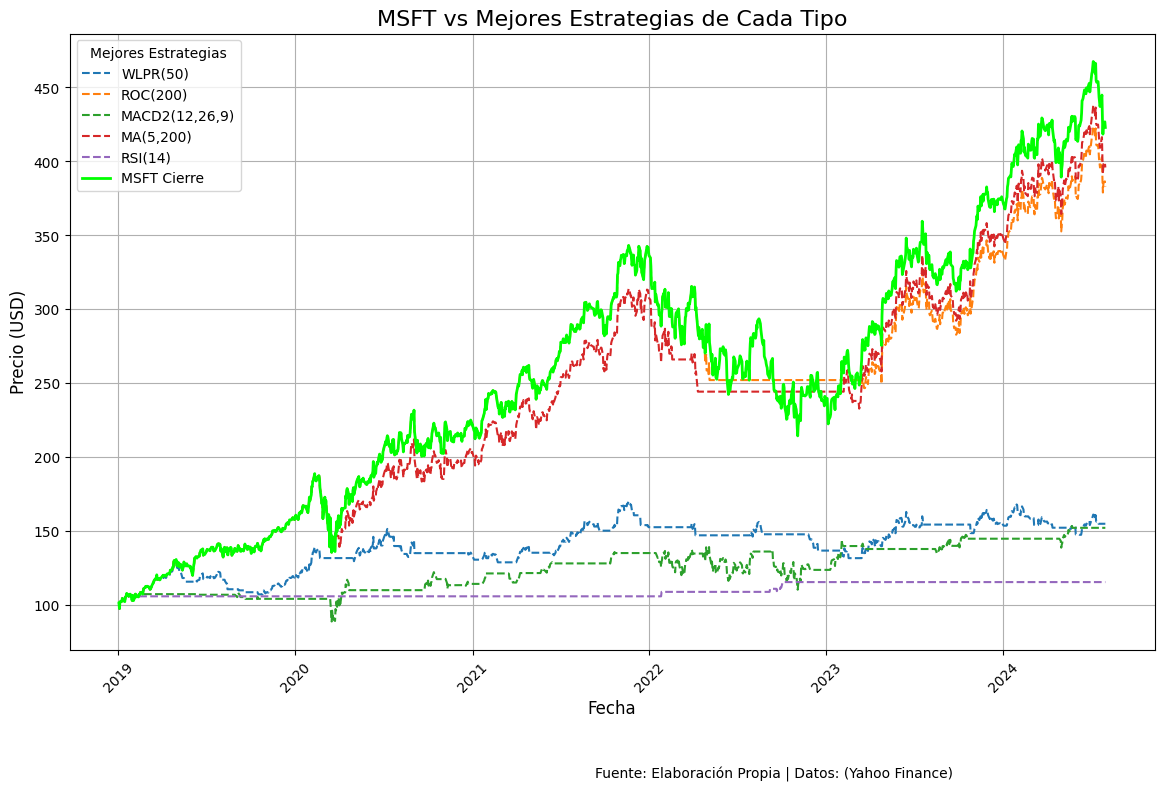
\includegraphics[width=0.9\linewidth]{grafico_mejores_estrategias_MSFT.png}
        \captionof{figure}{\footnotesize Este gráfico representa las mejores estrategias de cada tipo de indicador, y es aplicado al ticker 
        \emph{MSFT} correspondiente a Microsoft.}
                \end{minipage}
       
        \end{multicols}
    % Sección 2: Introducción
    \customsection{Introducción}
    \par
    \normalsize
    Esta tesis evalúa el poder predictivo de estrategias técnicas de tendencia y momentum sobre el mercado de acciones americanas.
    Utilizando indicadores técnicos, se implementaron modelos econométricos para predecir la dirección de las acciones en el 
    índice \textit{S\&P500} y evaluar su significancia. Los resultados sugieren que al menos la mitad de los indicadores son significativos, lo que valida el uso 
    de estas estrategias en la toma de decisiones de inversión.
    Ticker= accion de empresa

    En las últimas décadas, el mercado de acciones de EE. UU. ha experimentado cambios significativos, lo que ha llevado al
    desarrollo de estrategias técnicas como tendencia y momentum. Éstas estrategias, basadas en análisis de datos históricos, 
    son herramientas clave para predecir movimientos futuros en los precios de las acciones.
    % Sección 3: Metodología
    \customsection{Datos}
    \par
    %betas añadir
    Se utilizó una base de datos que abarca desde enero de 2019 hasta julio de 2024, con periodicidad de precios de cierre 
    diarios obtenidos de Yahoo Finance.\\
    % Tabla con minipage
    \begin{minipage}{.984\linewidth}
        \centering
        \vspace{1cm}
        \captionof{table}{Disección por \textit{Betas}.}
        \begin{tabular}{ccc}
            \toprule
            \textbf{Grupo} & \textbf{\textit{Beta}}  &\textbf{Empresas} \\
            \midrule
            1   &  $\beta < 0.5$  & 100                    \\
            2       & $0.5 \leq \beta \leq 1$  & 100  \\
            3      & $1 < \beta \leq 1.5$ & 100   \\
            4       & $1.5 < \beta $ & 100   \\
            5       & $\beta =N/A$  & 100  \\
            \bottomrule
            \vspace{.5cm}
        \end{tabular}
        \captionsetup{width=0.8\textwidth}  % Ajusta el ancho del pie de tabla
        \caption*{\footnotesize Valor $\beta$ corresponde a medida 
        de riesgo sistemática de correlación entre retornos de la acción 
        y el mercado. Obtenido desde base de datos de Yahoo Finance.
        }

        \end{minipage}
    \customsection{Metodología}
    \textbf{Indicadores técnicos:} Apartir de los indicadores técnicos se generan señales de compra (1) y venta (0) asumiendo que si el período anterior
     los que posteriormente generan señales binarias de 0 y 1.\\
     \begin{minipage}{.984\linewidth}
        \centering
        \vspace{1cm}
        \captionof{table}{Lista de indicadores técnicos.}
        \begin{tabular}{c p{10cm} l}
            \toprule
            \textbf{Indicador Técnico} & \textbf{Parámetros} & \textbf{Descripción}\\
            \midrule
             SMA & (1,50); (5,20); (1,150); (1,200); (2,200); (5,200);  & (Medias Móviles Simples)\\
             MACD & (12,26,9) & (Convergencia/Divergencia) \\
             ROC & (10); (50); (200) & (Tasa de Cambio) \\
             RSI & (14); (20); (50) & (Índice de Fuerza Relativa) \\
             WLPR & (14); (20); (50) &  (Williams \%R)\\
             Consolidated Technical Signal& SMA, ROC, RSi, WLPR, TODAS & \textbf{$***$} \\
            \bottomrule
        \end{tabular}
        \captionsetup{width=0.8\textwidth}  % Ajusta el ancho del pie de tabla
        \caption*{\footnotesize Donde $SMA(x,y)$ $x$ "SMA(x, y): 'x' es la media rápida e 'y' es la media lenta. MACD(12, 26, 9): '12' 
        es la EMA rápida, '26' la EMA lenta y '9' es la línea de señal. RSI(x): 'x' es el número de períodos. WLPR(x): 'x' representa el período de cálculo. 
        ROC(x): 'x' es el número de períodos para calcular el cambio de precio."\\
        \textbf{$***$} Se generon señales técnicas consolidadas basadas en cada estrategia con sus respectivos periodos, ademas una estrategia en donde se consolidan todos los indicadores. 
        Para cada combinación, generamos señales binarias: 1 cuando las señales activas son mas que la media de señales, y 0 en caso contrario. 
        Este procedimiento se aplica a cada indicador, permitiéndonos obtener señales consolidadas que refuerzan a validez de la estrategia técnica."
        }
        
    \end{minipage}
    \par
    \textbf{Modelos Econométricos:} Se construyeron varios modelos de regresión lineal para evaluar la capacidad predictiva de 
    estos indicadores técnicos. Las regresiones se estimaron con HAC según Newey-West (1987). Las señales técnicas se construyen 
    a base de los precios, arrojando 0 cuando la ventana corta es menor que la larga y 1 cuando es mayor. Tras obtener estas 
    variables dummy, se construyen las regresiones y se analiza la significancia de 
    las señales. 
    
    La ecuación general del modelo de regresión utilizado es la siguiente:

\begin{minipage}{.95\linewidth}
    \centering
    \vspace{1cm}
    \captionof{table}{Modelos de Regresión Utilizados.}
    \begin{tabular}{cl}
        \toprule

        \textbf{Modelo} & \multicolumn{1}{c}{\textbf{\textit{Regresión}}}   \\
        \midrule
        (Simple) & $R_{j,t} = \alpha + \gamma_1 \cdot Signal_{j,t-1}+\varepsilon_t$ \\
        (Rezago mínimo) & $R_{j,t} = \alpha + \gamma_1 \cdot Signal_{j,t-1} + \sum_{i=1}^{min(n)}  \gamma_{i+1} \cdot R_{j,t-i} +\varepsilon_t$ \\
        (Rezago máximo) & $R_{j,t} = \alpha + \gamma_1 \cdot Signal_{j,t-1} + \sum_{i=1}^{max(n)}  \gamma_{i+1} \cdot R_{j,t-i} +\varepsilon_t$ \\
        (Rezagos significativos) & $R_{j,t} = \alpha + \gamma_1 \cdot Signal_{j,t-1} + \sum_{i=1}^{n}  \gamma_{i+1} \cdot R_{j,t-i} +\varepsilon_t$ \\
        \bottomrule
    \end{tabular}
    \vspace{.3cm}
    \captionsetup{width=0.8\textwidth}  % Ajusta el ancho del pie de tabla
    \caption*{\footnotesize El modelo de regresión incluye rezagos del retorno \( R_{t-1}\)
    cuyo "n" es la lista de rezagos significativos para cada acción; Las señales técnicas \(Signal_{j,t-1}\) 
    son variables binarias obtenidas a través de los indicadores técnicos; El modelo ajusta los coeficientes $\gamma$ para cada acción.    }  % Pie de tabla
    \vspace{.5cm}
    \end{minipage}
       
                
                
%\columnbreak %para hacer el salto de la columna 
    % Sección 4:Resultados
    \customsection{Resultados}
    \par 
     \normalsize
    Como resultado de las regresiones de los 504 tickers, la base fue diseccionada tomando solo aquellas empresas 
    que han tenido un crecimiento constante durante los ultimos 5 años, ya que sus retornos reflejan esta información, 
    haciendo que nuesto modelo fuera de muestra presente mayor significancia y probabilidades de predecir con éxito el 
    retorno de estas acciones.
    

    \vspace{1cm}
    \begin{comment}
        
        % Tabla con minipage
        \begin{minipage}{,984\linewidth}
        \centering
        \captionof{table}{Resultados de los coeficientes para diferentes benchmarks.}
        \begin{tabular}{ccccccc}
        \toprule
        \textbf{Grupo} & \textbf{pollo} & \textbf{Leyton} & \textbf{Por-ano} & \textbf{Sacamos oro} & \textbf{detroit} \\
        \midrule
        1   & 1.217*  & 3.684*** & 2.45** & 0.074  & 1.473*  \\
        2       & 1.535*  & 2.927**  & 2.379* & 0.149  & 1.586** \\
        3       & 1.52*   & 2.903**  & 2.374* & 0.144  & 1.579*  \\
        4       & 1.213*  & 3.576**  & 2.344* & 0.1427 & 1.625** \\
        5    & 1.131*  & 3.824*** & 2.489** & 0.028  & 1.456** \\
        \bottomrule
        \vspace{.5cm}
    \end{tabular}
\end{minipage}
\end{comment}
    % Sección 5: Conclusiones
    \customsection{Conclusiones}
    \par
    \indent La investigación valida el uso de estrategias de tendencia y momentum para predecir el mercado de acciones 
    estadounidense. Estas herramientas son valiosas para los inversores que buscan optimizar su toma de decisiones en un 
    entorno bursátil dinámico. 
    % Sección 6: Referencias   
    \customsection{Referencias}
    \par
         \begin{itemize}
            \vspace{-,5 cm}
            \item Gradojevic (2023) Forecasting Bitcoin with technical analysis: A not-so-random forest?
            \vspace{-1 cm}
            \item Ifleh et al. (2023). Stock price indices prediction combining deep learning algorithms and selected technical 
            indicators based on correlation
            \vspace{-1 cm}
            \item Jegadeesh, N., y Titman, S. (1993). Returns to buying winners and selling losers: Implications for stock 
            market efficiency.
            \vspace{-1 cm}
            \item Lim, B. Y., Wang, J. G., y Yao, Y. (2018). Time-Series Momentum in nearly 100 years of stock returns.            
            \vspace{-1 cm}
            \item Subrahmanyam, A. (2018). Equity market momentum: A synthesis of the literature and suggestions for future work.
            \vspace{-1 cm}
            \item Wu et al. (2020) Adaptive stock trading strategies with deep reinforcement learning methods
        \end{itemize}
        
    
    
    

    
\end{multicols}
\end{document}
